\documentclass[a4paper,10pt]{book}
\usepackage[utf8]{inputenc}
\usepackage{graphicx}
\usepackage{amsmath}
\usepackage{amsfonts}
\usepackage{url}

%opening
\title{}
\author{}

\begin{document}
\chapter{18 de setembro}

\section{Definição}

A transformada de Laplace é definida como:
$$F(s)=\mathcal{L}\{ f(t)\} := \int_0^\infty f(t)e^{-st}dt,~~\Re(s)>s_0$$

 Exemplo:
 
 $$f(t)=1$$
 \begin{eqnarray*}
  F(s) &=& \int_0^\infty f(t)e^{-st}dt\\
  &=&\int_0^\infty e^{-st}dt\\
  &=&\left.\frac{e^{-st}}{-s}\right|_{t=0}^{t \to \infty}\\
  &=& \frac{0-1}{-s}=\frac{1}{s}, ~~s>0.
 \end{eqnarray*}
% 

Exemplo:
 $$f(t)=e^{as}$$
 
 
 \begin{eqnarray*}
  F(s) &=& \int_0^\infty f(t)e^{-st}dt\\
  &=&\int_0^\infty e^{at}e^{-st}dt\\
    &=&\int_0^\infty e^{(a-s)t}dt\\
    &=&\left.\frac{e^{(a-s)t}}{a-s}\right|_0^\infty\\
    &=&\frac{0-1}{a-s}\\
    &=&\frac{1}{s-a},~~~s>a.
 \end{eqnarray*}
% 
% 
% 
 \section{Propriedade da linearidade}
% 
 $$\mathcal{L}\{\alpha f(t)+\beta g(t)\}=\alpha\mathcal{L}\{ f(t)\}+\beta\mathcal{L}\{ g(t)\}$$

 exemplo:
 
 \begin{eqnarray*}
\mathcal{L}\{3+2 e^{t}\}&=&3\mathcal{L}\{ 1\}+2\mathcal{L}\{ e^t\} \\
&=&\frac{3}{s}+\frac{2}{s-1}
 \end{eqnarray*}

 % 
% 
 \section{Propriedade da derivada}
 $$\mathcal{L}\{f'(t)\}=s\mathcal{L}\{ f(t)\}-f(0)$$

 Exemplo:
 
 $$f(t)=t$$
 $$f'(t)=1$$
 
 $$\mathcal{L}\{1\}=s\mathcal{L}\{ t\}-0$$
 $$\mathcal{L}\{ t\} = \frac{1}{s^2}$$


  Exemplo:
 
 $$f(t)=t^2$$
 $$f'(t)=2t$$
 
 $$\mathcal{L}\{2t\}=s\mathcal{L}\{ t^2\}-0$$
 $$\mathcal{L}\{ t^2\} = \frac{2}{s^3}$$

 
 Analogamente:
 $$\mathcal{L}\{ t^3\} = \frac{6}{s^4}$$

  $$\mathcal{L}\{ t^n\} = \frac{n!}{s^{n+1}}$$
  
  
  
  Aplicação:
  
  $$f'(t)+f(t) = 1$$
  com $f(0)=1$.

  Aplicando a transformada de Laplace, temos:
  
  $$\left[sF(s)-f(0)\right]+F(s)=\frac{1}{s}$$
  
  $$F(s)(s+1) = \frac{1}{s}+1$$
  
  $$F(s) = \frac{1}{s(s+1)}+\frac{1}{(s+1)}$$
  
  $$F(s) = \frac{1+s}{s(s+1)}=\frac{1}{s}$$
  
  $$f(t)=1$$
  
  OBS: $f(t)=1, t\neq 2$,  $f(2)=0$.
  
  
  \chapter{21 de setembro}

  \section{A transformada inversa}
  
  Se $\mathcal{L}\{f(t)\}=F(s)$, dizemos que $f(t)$ é a transformada inversa de $F(s)$:
  $$\mathcal{L}^ {-1}(F(s))=f(t)$$
  
  \section{Propriedade da derivada - derivada segunda}
 Vimos a propriedade da derivada:
    $$\mathcal{L}\{f'(t)\}=s\mathcal{L}\{ f(t)\}-f(0)$$
 
 Agora aplicamos à derivada da função $f'(t)$:
 \begin{eqnarray*}
 \mathcal{L}\{f''(t)\}&=&s\mathcal{L}\{ f'(t)\}-f'(0)\\
 &=&s\left[sF(s)-f(0)\right]-f'(0)\\
 &=&s^2F(s)-sf(0)-f'(0)\\
 \end{eqnarray*}

 Analogamente:
 \begin{eqnarray*}
 \mathcal{L}\{f'''(t)\}
  &=&s^3F(s)-s^2f(0)-sf'(0)-f''(0)\\
 \end{eqnarray*}

 
 % 
 Exemplo:
 \begin{eqnarray*}f(t)&=&\cos(\omega t)\\
 f'(t)&=&-\omega\sin(\omega t)\\
 f''(t)&=&-\omega^2\cos(\omega t)
 \end{eqnarray*}
 
 isto é:
 $$f''(t)=-\omega^2f(t)$$
 Aplicando a transformada de Laplace, temos:
 \begin{eqnarray*}
 \mathcal{L}\{f''(t)\}&=&-\omega^2\mathcal{L}\{ f(t)\}.
 \end{eqnarray*}
 Usamos a propriedade da derivada (segunda):
 \begin{eqnarray*}
 s^2F(s)-sf(0)-f'(0)&=&-\omega^2F(s)
 \end{eqnarray*}
 isto é:
 \begin{eqnarray*}
 (s^2+\omega^2)F(s)=sf(0)+f'(0)=s
 \end{eqnarray*}
 Portanto:
 $$F(s)=\mathcal{L}\{\cos(\omega t)\}=\frac{s}{s^2+\omega^2},~~s>0$$
% 
 Analogamente, temos:
 $$\mathcal{L}\{\sin(\omega t)\}=\frac{w}{s^2+\omega^2}$$
 
 \section{Método das frações parciais para calcular transformadas inversas
 }
% * Ler seção 3.4 do livro. %https://www.ufrgs.br/reamat/TransformadasIntegrais/livro-tl/apdleatdd-mx00e9todo_das_frax00e7x00f5es_parciais_para_calcular_transformadasinversas.html
% 
 \begin{eqnarray*}F(s)&=&\frac{s^2-6s+4}{s^3-3s^2+2s}\\
 &=&\frac{s^2-6s+4}{s(s^2-3s+2)}\\
 &=&\frac{s^2-6s+4}{s(s-1)(s-2)}\\
 &=&\frac{A}{s}+\frac{B}{s-1}+\frac{C}{s-2}
 \end{eqnarray*}
% 
 O teorema das frações parciais garante que existem constantes $A$, $B$ e $C$ tais que:
 \begin{eqnarray}\label{eq_or_fp}\frac{s^2-6s+4}{s(s-1)(s-2)}
 &=&\frac{A}{s}+\frac{B}{s-1}+\frac{C}{s-2}
 \end{eqnarray}
 para todo $s$ complexo.

 
Primeiro multiplicamos (\ref{eq_or_fp}) por $s$:
\begin{eqnarray*}\frac{s^2-6s+4}{(s-1)(s-2)}
 &=&A+\frac{Bs}{s-1}+\frac{Cs}{s-2}
 \end{eqnarray*}
Substituindo $s$ por $0$, temos:
\begin{eqnarray*}\frac{4}{(-1)(-2)}
 =A~~~\Longrightarrow ~~ A=2
 \end{eqnarray*}

 
Agora multiplicamos a expressão (\ref{eq_or_fp}) por $s-1$:
% 
 \begin{eqnarray*}\frac{s^2-6s+4}{s(s-2)}
 &=&\frac{A(s-1)}{s}+{B}+\frac{C(s-1)}{s-2}
 \end{eqnarray*}

 Substituindo $s$ por 1, temos:

  \begin{eqnarray*}\frac{1-6+4}{1(1-2)}
 =B~~~\Longrightarrow ~~B = 1
 \end{eqnarray*}

 Finalmente multiplicamos (\ref{eq_or_fp}) por $s-2$:
 % 
 
 \begin{eqnarray*}\frac{s^2-6s+4}{s(s-1)}
 &=&\frac{A(s-2)}{s}+\frac{B(s-2)}{s-1}+{C}
 \end{eqnarray*}
E substuimos por $s=2$:

 \begin{eqnarray*}\frac{4-12+4}{2(2-1)}
 ={C}~~~\Longrightarrow ~~C = -2
 \end{eqnarray*}

 
 \begin{eqnarray}F(s)&=&\frac{s^2-6s+4}{s(s-1)(s-2)}\\
 &=&\frac{2}{s}+\frac{1}{s-1}-\frac{2}{s-2}
 \end{eqnarray}
 
 Olhanda na tabela, encontramos:
 $$f(t)=2+e^t-2e^{2t},~~t\geq 0$$
 Tabela com item 1 e item 7 com $a=1$ e $a=2$.
 
 {\bf Obs:}
 
 $$F(s)=\frac{s}{(s^2+1)(s-2)^3}=\frac{A+Bs}{s^2+1}+\frac{C}{(s-2)}+\frac{D}{(s-2)^2}+\frac{E}{(s-2)^3}$$
 % 
  \section{Propriedade de translação no eixo s}
% 
  Se $F(s)$ é a transformada de Laplace de $f(t)$ definida para $s>s_0$, então $e^{at}f(t)$ é a transformada inversa de $F(s-a)$, isto é
  \begin{equation*}
  \mathcal{L}\left\{e^{at}f(t)\right\} =F(s-a),\qquad s>s_0+a
  \end{equation*}
  A demostração vem da aplicação da definição da transformada de Laplace $F(s-a)$:
 \begin{eqnarray*}
   F(s-a)&=&\int_0^\infty f(t)e^{-(s-a)t}dt\\
  &=&\int_0^\infty f(t)e^{at}e^{-st}dt\\
&=&\int_0^\infty \left(f(t)e^{at}\right)e^{-st}dt\\
    &=&\mathcal{L}\left\{e^{at}f(t)\right\}
   \end{eqnarray*}

{\bf Exemplo:}
$$\mathcal{L}\left\{t^2\right\}=\frac{2}{s^3}$$
   
$$\mathcal{L}\left\{t^2e^{at}\right\}=\frac{2}{(s-a)^3}$$
   
   %  
  \section{Oscilador harmônico}
%  %https://www.ufrgs.br/reamat/TransformadasIntegrais/livro-tl/apdtedtd-aplicax00e7x00e3o_oscilador_harmx00f4nico.html
$$F(s)=\frac{1}{ms^2+\gamma s+ \kappa}$$


Caso $m=1$, $\gamma=0$, $\kappa =4$:

$$F(s)=\frac{1}{s^2+ 4}=\frac{1}{s^2+ 2^2}$$

$$f(t)=\frac{1}{2}\sin(2t)$$

Caso $m=1$, $\gamma=2$, $\kappa =5$:

\begin{eqnarray*}F(s)&=&\frac{1}{s^2+2 s+ 5}\\
&=&\frac{1}{\underbrace{(s+1)^2}_{s^2+2s+1}+4}\\
&=&\frac{1}{(s+1)^2+2^2}\\
&=&G(s+1)
 \end{eqnarray*}
onde $G(s)=\frac{1}{s^2+2^2}$
 
 Como $$g(t)=\mathcal{L}^{-1}\{G(s)\}=\frac{1}{2}\sin(2t)$$ $$f(t)=\frac{1}{2}e^{-t}\sin(2t)$$
Onde usamos o produto notável: $$(s+a)^2=s^2+2as+a^2.$$
 
 Caso $m=1$, $\gamma=3$, $\kappa=2$:
\begin{eqnarray*}F(s)&=&\frac{1}{s^2+3 s+ 2}\\
F(s)&=&\frac{1}{(s+1)(s+2)}\\
 \end{eqnarray*}

 Usando a tabela, encontramos:
 $$f(t)=e^{-t}-e^{-2t}$$
 
 Pergunta: Quantas vezes $f(t)$ para por zero para $t\geq 0$.
 $$f(t)=e^{-t}-e^{-2t}=0$$
 $$e^{-t}(1-e^{-t})=0$$
  Assim $f(t)=0$ se e somente se $e^{-t}=1$, i.e., $t=0$.
  
  
  \chapter{23 de setembro}
  \section{Exemplo de cálculo de transformada de Laplace usando função de Heaviside}
  
 Representar algebricamente em termos da função de Heaviside a função dada no gráfico da figura \ref{fig_Heaviside_4}.
\begin{figure}[!ht]
\begin{center}

\includegraphics{figs/figura_8}\end{center}
\caption{\label{fig_Heaviside_4}}
\end{figure} 
 Observe que podemos representar $f(t)$ da seguinte forma:
 \begin{equation}
  f(t)=\left\{ \begin{array}{ll} 0, &t<1\\2,&1<t<3\\-3,& 3<t<5\\0,&t>5. \end{array}\right.
 \end{equation}
 Para representar em termos da função de Heaviside, olhe para o gráfico pensando em dois pulsos: $2(u(t-1)-u(t-3))$ e $-3(u(t-3)-u(t-5))$. A soma deles é a função desejada:
 \begin{equation}
 f(t)=2(u(t-1)-u(t-3))-3(u(t-3)-u(t-5)).
 \end{equation}

 \begin{equation}
 f(t)=2u(t-1)-5u(t-3)+3u(t-5).
 \end{equation}
 \begin{figure}[!ht]
\begin{center}

\includegraphics{figs/figura_8}\end{center}
\caption{\label{fig_Heaviside_4}}
\end{figure} 
 $$F(s)=\frac{2e^{s}-5e^{-3s}+3e^{-5s}}{s}$$
onde usamos que
$$\mathcal{L}\{u(t-a)\}=\frac{e^{-as}}{s}$$
O que vamos provar agora.  
 \section{Transformada de Laplace da Heaviside}
% 
 $$f(t)=u(t-a), ~~a>0$$
% 
 \begin{eqnarray*}
  F(s)&=&\int_0^\infty f(t)e^{-st}dt\\
  &=&\int_0^\infty u(t-a)e^{-st}dt\\
&=&\int_0^a \underbrace{u(t-a)}_{0}e^{-st}dt + \int_a^\infty \underbrace{u(t-a)}_{1}e^{-st}dt\\
&=& \int_a^\infty e^{-st}dt\\
&=&\left.\frac{e^{-st}}{-s}\right|_{t=a}^\infty\\
&=&\frac{e^{-as}}{s},~~s>0
\end{eqnarray*}
% 
 \section{Propriedade do deslocamento no tempo}
% 
   Se $F(s)$ é a transformada de $f(t)$, então $f(t-a)u(t-a)$ é a transformada inversa de $e^{-as}F(s)$, isto é
 \begin{equation}
 \mathcal{L}\left\{u(t-a)f(t-a)\right\} =e^{-as}F(s),\qquad a>0
 \end{equation}
 ou
 \begin{equation}{\label{eq_trans_t_inv}}
 \mathcal{L}^{-1} \left\{e^{-as}F(s)\right\} =u(t-a)f(t-a),\qquad a>0.
 \end{equation} 
%  
 Dem: Aplicamos a definição da transformada de Laplace e obtemos:
  \begin{eqnarray*}
  \mathcal{L}\left\{u(t-a)f(t-a)\right\}&=&\int_0^\infty u(t-a)f(t-a)e^{-st}dt\\
  &=&\int_0^a \underbrace{u(t-a)}_{0}f(t-a)e^{-st}dt+\int_a^\infty \underbrace{u(t-a)}_{1}f(t-a)e^{-st}dt\\
  &=&\int_a^\infty f(t-a)e^{-st}dt,
  \end{eqnarray*}
  pois $u(t-a)$ é zero no intervalo $[0,a)$ e um no intervalo $(a,\infty)$. Depois usamos a mudança de variável $v=t-a$ na última integral:
  \begin{equation*}
  \int_a^\infty f(t-a)e^{-st}dt=\int_0^\infty f(v)e^{-s(v+a)}dv=e^{-as}\int_0^\infty f(v)e^{-sv}dv.
  \end{equation*}
  Logo,
  \begin{equation}
  \mathcal{L}\left\{u(t-a)f(t-a)\right\}=e^{-as}\mathcal{L}\left\{f(t)\right\}=e^{-as}F(s).
  \end{equation}
% 
  Observe que tomando $f(t)=1$ na propriedade do deslocamento, temos:
  \begin{equation}{\label{Heaviside_trans_1}}
  \mathcal{L}\left\{1~\!u(t-a)\right\} =\frac{e^{-as}}{s},\qquad a>0
  \end{equation}
  que coincide com a fórmula da transformada de Laplace da Heaviside. %
  Quando $a=0$ na equação acima, recaímos no item 1 da tabela de transformadas.
 
  

{\bf Exemplo} Aplicando diretamente a propriedade do deslocamento em $t$ e usando que $\mathcal{L}\{t^2\}=\frac{2}{s^3}$, calculamos a transformada inversa de Laplace de $e^{-3s}\frac{2}{s^3}$:
  \begin{equation}
  \mathcal{L}^{-1}\left\{e^{-3s}\frac{2}{s^3}\right\}=u(t-3)(t-3)^2.
  \end{equation}
Cuidado:
  \begin{equation}
  u(t-3)(t-3)^2 \neq u(t-3)t^2.
  \end{equation}

  %  
%  
%   
   {\bf Exemplo:}
   Vamos calcular a transformada inversa de Laplace da função
  \begin{equation}
  F(s)=e^{-s}\frac{1}{(s+1)^2-1}.
  \end{equation}
{\bf Obs:} As raizes do denominador são:
$$(s+1)^2-1=0$$
  $$(s+1)^2=1$$
  $$(s+1) = \pm 1$$
  $$s = -1\pm 1$$
  
    Primeiro calculamos a transformada de $\frac{1}{(s+1)^2-1}$ usando a propriedade.
   \begin{eqnarray*}
   \mathcal{L}^{-1}\left\{\frac{1}{(s+1)^2-1}\right\}&=&e^{-t}\sinh(t)\\
   &=&e^{-t}\left(\frac{e^{t}-e^{-t}}{2}\right)\\
   &=&\frac{1-2e^{-2t}}{2}
 \end{eqnarray*}
  Depois usamos a propriedade  para concluir
  \begin{equation}
  \mathcal{L}^{-1}\left\{e^{-s}\frac{1}{(s+1)^2-1}\right\}=u(t-1)\mathcal{L}^{-1}\left\{\frac{1}{(s+1)^2-1}\right\}
  _{t\to t-1}=u(t-1)e^{-(t-1)}\sinh(t-1).
   \end{equation}
% % 
%   
%   
%   
 \section{A propriedade da transformada de Laplace da integral de uma função}
  Se $F(s)$ é a transformada de Laplace de uma função contínua por partes $f(t)$, então $\int_0^tf(\tau)d\tau$ é a transformada inversa de $\frac{1}{s}F(s)$, isto é
 \begin{equation}{\label{eq_trans_int}}
 \mathcal{L}\left\{\int_0^tf(\tau)d\tau\right\} =\frac{1}{s}F(s),
 \end{equation}
 ou
 \begin{equation}{\label{eq_trans_int_inv}}
 \mathcal{L}^{-1} \left\{\frac{1}{s}F(s)\right\} =\int_0^tf(\tau)d\tau.
 \end{equation} 
% 
Dem: Seja $g(t)=\int_0^tf(\tau)d\tau$. Então $g'(t)=f(t)$. Aplicamos a propriedade da transformada da derivada  e temos:
 \begin{equation}
 \mathcal{L}\{g'(t)\}=s\mathcal{L}\{g(t)\}-g(0).
 \end{equation}
 Usando o fato que $g(0)=0$, temos
 \begin{eqnarray*}
 \mathcal{L}\left\{\int_0^tf(\tau)d\tau\right\}&=&\mathcal{L}\left\{g(t)\right\}\\
 &=&\frac{1}{s}\mathcal{L}\{g'(t)\}\\
 &=&\frac{1}{s}\mathcal{L}\{f(t)\}\\
 &=&\frac{1}{s}F(s).
 \end{eqnarray*}
% 
% 
  
  \chapter{Dia 25 de setembro}
  \section{Oscilador harmônico - regime de amortecimento}
  
  Ver aula no 
  \url{https://colab.research.google.com/drive/197QbUeLlV2GEulEhjyVfpBeNRngxLls3}
  
  \noindent Mais exemplos de PVI em:
  \url{https://colab.research.google.com/drive/1MTC1GSOP_DLPYZusqohP9DcaWr_ab-UX}
  
  
   \section{Delta de dirac}
   Muitos fenômenos físicos exigem a representação de uma força muito grande em um intervalo de tempo muito pequeno, por exemplo:
 \begin{itemize}
  \item um circuito elétrico recebe uma força eletromotriz grande em um curto intervalo de tempo.
  \item um sistema massa-mola é atingido por uma martelo.
  \item uma bola de futebol parada recebe um chute, ou seja, uma força quase instantânea, que a coloca em movimento.
  \item um avião é atingido por um raio.
 \end{itemize}
 Para representar essa força, vamos tomar a função pulso unitário em um curto intervalo de tempo $[-\epsilon,\epsilon]$ em torno da origem, isto é, um pulso com integral unitária:
 \begin{equation}
 \delta_\epsilon(t)=\frac{1}{2\epsilon}\left(u(t+\epsilon)-u(t-\epsilon)\right)=\left\{\begin{array}{ll}0,&t<-\epsilon\\ \frac{1}{2\epsilon},&-\epsilon<t<\epsilon\\0,&t>\epsilon.\end{array}\right.
 \end{equation}
 Um pulso unitário em torno de $t=a$ é representado por
 \begin{equation}{\label{def_delta_dirac}}
 \delta_\epsilon(t-a)=\frac{1}{2\epsilon}\left(u(t-(a-\epsilon))-u(t-(a+\epsilon))\right)=\left\{\begin{array}{ll}0,&t<a-\epsilon\\ \frac{1}{2\epsilon},&a-\epsilon<t<a+\epsilon\\0,&t>a+\epsilon.\end{array}\right.
 \end{equation}
 Observe que $\int_{-\infty}^\infty\delta_\epsilon(t-a)=1$ para qualquer $\epsilon>0$. A figura \ref{fig_delta_dirac} apresenta o gráfico de $\delta_\epsilon(t-a)$ para $a>0$ e $\epsilon=1$, $\epsilon=\frac{1}{2}$, $\epsilon=\frac{1}{4}$, $\epsilon=\frac{1}{8}$ e $\epsilon=\frac{1}{12}$.
 A função que representa uma grande força instantânea é chamada de {\bf função impulso} ou {\bf função Delta de Dirac} e pode ser definida pelo limite das funções pulsos:
 \begin{equation}
 \delta(t-a)=\lim_{\epsilon\to 0}\delta_\epsilon(t-a).
 \end{equation}
 Este limite não pode ser interpretado pontualmente, isto é, como o limite usual de funções reais, mas apenas no contexto de uma integral, como veremos.
 A figura \ref{fig_delta_dirac} apresenta o gráfico de $\delta_\epsilon(t-a)$ quando $\epsilon$ diminui e uma representação gráfica para $\delta(t-a)$.
% 
%   
 \begin{figure}[!ht]
 \begin{center}
% 
 \includegraphics{figs/figura_1}\hspace{20pt}
 \includegraphics{figs/figura_2}\hspace{20pt}
 \includegraphics{figs/figura_3}
 
 \includegraphics{figs/figura_4}\hspace{20pt}
 \includegraphics{figs/figura_5}\hspace{20pt}
 \includegraphics{figs/figura_6}
 \end{center}
 \caption{\label{fig_delta_dirac}}
 \end{figure}
% 
 {\bf Obs:}A função delta de Dirac pode ser definida como limite de outras sequências de funções com propriedades análogas a sequência de pulsos. Por exemplo, podemos definir $\delta(t)$ como limite das funções
 \begin{equation}
 f_\epsilon(t)=\frac{1}{\epsilon\sqrt{\pi}}e^{-\frac{t^2}{\epsilon^2}}
 \end{equation}
% 
% 
% 
 A função Impulso é zero em todo ponto, exceto em $t=a$:
 \begin{equation}
 \delta(t-a)=\left\{\begin{array}{ll}0,&t\neq a\\\infty,&t=a  \end{array}\right.
 \end{equation}
 e
 \begin{equation}
 \int_{-\infty}^\infty\delta(t-a)dt=1
 \end{equation}
 A função Delta de Dirac deve ser sempre compreendida como o limite de funções reais no contexto de uma integração, isto conduz à chamada  {\bf propriedade da filtragem}, que define totalmente a Delta da Dirac:
 Se $f(t)$ for um função contínua em torno de $t=a$, então
 \begin{equation}{\label{prop_filtragem_dirac}}
 \int_{-\infty}^\infty \delta(t-a)f(t)dt=f(a). 
 \end{equation}
 Para chegar a esta conclusão, definimos $F(t)=\int_a^t f(\tau)d\tau$ e calculamos:
 \begin{eqnarray*}
 \int_{-\infty}^\infty \delta(t-a)f(t)dt&=&\lim_{\varepsilon\to 0+}
 \int_{-\infty}^\infty \delta_\varepsilon(t-a)f(t)dt\\
 &=&\lim_{\varepsilon\to 0+}\frac{1}{2\varepsilon}\int_{-a+\varepsilon}^{a+\varepsilon} f(t)dt\\
 &=&\lim_{\varepsilon\to 0+}\frac{F(\varepsilon)-F(-\varepsilon)}{2\varepsilon}\\
 &=&F'(0)=f(a).
 \end{eqnarray*}
 \subsection{Delta de Dirac como derivada distribucional da função Heaviside}
 Na equação (\ref{def_delta_dirac}) definimos a função Delta de Dirac como
 \begin{equation}
 \delta(t-a)=\lim_{\epsilon\to 0}\frac{1}{2\epsilon}\left(u(t-(a-\epsilon))-u(t-(a+\epsilon))\right).
 \end{equation}
 Por outro lado, usamos a definição de derivada para escrever
 \begin{equation}
 \lim_{\epsilon\to 0}\frac{1}{2\epsilon}\left(u((t-a)+\epsilon))-u((t-a)-\epsilon))\right)=\frac{d}{dt}u(t-a)
 \end{equation}
 ou seja,
 \begin{equation}
 \delta(t-a)=\frac{d}{dt}u(t-a).
 \end{equation}
 Observe que as funções de Heaviside e de Dirac não são funções no sentido do cálculo diferencial e integral. Naturalmente, a derivada acima também vale somente num sentido generalizado, mas é coerente quando olhamos a função de Heaviside como limite de funções rampas (ver figura \ref{fig_Heaviside_1}), pois na origem a derivada tende ao infinito.
 A transformada de Laplace de função Delta de Dirac é obtido pela propriedade da filtragem dada na equação (\ref{prop_filtragem_dirac}):
 \begin{equation}{\label{prop_trans_delta_dirac}}
 \mathcal{L}\{\delta(t-a)\}=\int_0^\infty \delta(t-a)e^{-st}dt=e^{-as}.
 \end{equation}

 
 
 \chapter{Aula do dia 28/09}
  


\section{Circuito RLC}{\label{sec_circ_2}}
Ver \url{https://colab.research.google.com/drive/1R3rCOc8zv70rSwCf7W30yQlleP6J2Mf2}

Considere o circuito Resistor/Capacitor/Indutor representado na figura \ref{fig_circ_2} com uma tensão $V(t)$ aplicada do tipo pulso,
\begin{equation}
V(t)=V_0\left(u(t-a)-u(t-b)\right).
\end{equation}
\begin{figure}[!ht]
\begin{center}

\includegraphics{figs/figura_7_RLC}\end{center}
\caption{\label{fig_circ_2}}
\end{figure} 
 O modelo para a corrente $i(t)$ obedece a lei de Kirchoff:
 \begin{equation}{\label{modelo_corrente}}
 Li'(t)+ Ri(t)+\frac{1}{C}q(t)=V_0\left(u(t-a)-u(t-b)\right),
 \end{equation}
 onde $q(t)$ é a carga no capacitor, $\frac{1}{C}q(t)$ é a tensão no capacitor de capacitância $C$, $Ri(t)$ é a tensão no resistor de resistência $R$ e $Li'(t)$ é a tensão no indutor de indutância $L$. Considere as condições iniciais $i(0)=0$ e $q(0)=0$.
 Dado que $\frac{dq(t)}{dt}=i(t)$, derivamos a equação do circutio para obter a seguinte equação diferencial:
 \begin{equation}{\label{modelo_corrente_2}}
 Li''(t)+ Ri'(t)+\frac{1}{C}i(t)=V_0\left(\delta(t-a)-\delta(t-b)\right),
 \end{equation}
 onde usamos que a derivada da função de Heaviside é a função delta de Dirac. As condições iniciais para a equação (\ref{modelo_corrente_2}) são $i'(0)=0$ e $i(0)=0$. Com o objetivo de resolver a problema de valor inicial, aplicamos a transformada de Laplace para obter a equação subsidiária
 \begin{equation*}
 Ls^2I(s)+ RsI(s)+\frac{1}{C}I(s)=V_0\left(e^{-as}-e^{-bs}\right),
 \end{equation*}
 que tem solução
% 
% 
 \begin{eqnarray*}
 I(s)&=&\frac{V_0\left(e^{-as}-e^{-bs}\right)}{Ls^2+Rs+\frac{1}{C}}\\
 &=&\frac{1}{L}\frac{V_0\left(e^{-as}-e^{-bs}\right)}{\left(s+\frac{R}{2L}\right)^2-\left(\frac{R}{2L}\right)^2+\frac{1}{LC}}\\
 &=&\frac{V_0}{L}\left[\frac{e^{-as}}{\left(s+\frac{R}{2L}\right)^2+\eta}-\frac{e^{-bs}}{\left(s+\frac{R}{2L}\right)^2+\eta}\right]
 \end{eqnarray*}
 onde
 \begin{equation}
 \eta=\frac{1}{LC}-\left(\frac{R}{2L}\right)^2.
 \end{equation}
 Vamos exemplificar os casos subamortecido, superamortecido e criticamente amortecido tomando $V_0=10V$, $a=1$ e $b=5$:
 \begin{itemize}
  \item Caso subamortecido ($\eta>0$): escolhemos o caso onde $L=1\ \!$H, $C=\frac{1}{10}\ \!$F e $R=2\Omega$. Nesse caso
  \begin{equation}
  I(s)=10\left[\frac{e^{-s}}{\left(s+1\right)^2+9}-\frac{e^{-5s}}{\left(s+1\right)^2+9}\right].
  \end{equation}
  Logo,
  \begin{equation}
  i(t)=\frac{10}{3}\left(u(t-1)e^{-(t-1)}\sin\left(3 (t-1)\right)-u(t-5) e^{-(t-5)}\sin\left(3 (t-5)\right)\right).
  \end{equation}
  O gráfico da corrente é apresentado na figura \ref{fig_circ_RCL_1}.
 \begin{figure}[!ht]
 \begin{center}
% 
 \includegraphics{figs/figura_8}\end{center}
 \caption{\label{fig_circ_RCL_1}}
 \end{figure}
  \item Caso superamortecido ($\eta<0$): escolhemos o caso onde $L=1\ \!$H, $C=1\ \!$F e $R=4\Omega$. Nesse caso
  \begin{equation}
  I(s)=10\left[\frac{e^{-s}}{\left(s+2\right)^2-3 }-\frac{e^{-5s}}{\left(s+2\right)^2-3}\right].
  \end{equation}
  Logo,
  \begin{eqnarray*}
  i(t)&=&10\left(u(t-1)\frac{e^{-2(t-1)}}{ \sqrt{3}}\sinh\left(\sqrt{3} (t-1)\right)-u(t-5)\frac{e^{-2(t-5)}}{\sqrt{3} }\sinh\left(\sqrt{3}  (t-5)\right)\right)\\
  &=&\frac{5}{\sqrt{3}}u(t-1)\left(e^{\left(\sqrt{3}-2\right) (t-1)}-e^{-\left(\sqrt{3}+2\right) (t-1)}\right)+\\
  &+&\frac{5}{\sqrt{3}}u(t-5)\left(e^{\left(\sqrt{3}-2\right) (t-5)}-e^{-\left(\sqrt{3}+2\right) (t-5)}\right)
  \end{eqnarray*}
  O gráfico da corrente é apresentado na figura \ref{fig_circ_RCL_2}.
 \begin{figure}[!ht]
 \begin{center}
 
 \includegraphics{figs/figura_9}\end{center}
 \caption{\label{fig_circ_RCL_2}}
 \end{figure}
 \item Caso criticamente amortecido ($\eta=0$): escolhemos o caso onde $L=1\ \!$H, $C=1\ \!$F e $R=2\Omega$. Nesse caso
  \begin{equation}
  I(s)=10\left[\frac{e^{-s}}{\left(s+1\right)^2}-\frac{e^{-5s}}{\left(s+1\right)^2}\right].
  \end{equation}
  Logo,
  \begin{equation}
  i(t)=10\left(u(t-1)e^{-(t-1)} (t-1)-u(t-5)e^{-(t-5)} (t-5)\right).
  \end{equation}
O gráfico da corrente é apresentado na figura \ref{fig_circ_RCL_3}.
 \begin{figure}[!ht]
 \begin{center}
 \includegraphics{figs/figura_10}\end{center}
 \caption{\label{fig_circ_RCL_3}}
 \end{figure}
 \end{itemize}
% 
% 
 \section{Exemplo}
 Resolva o PVI $\displaystyle \left\{
                               \begin{array}{ll}
                                 y'' + 3y'+2y = \delta(t-5) - u(t-10)\\
                                 y(0) = 0, \quad y'(0)=1/2
                                 \end{array}
                             \right.$
 
 \begin{enumerate}
  \item Aplicar a transformada de Laplace e substituir as condições iniciais
  $$
  s^2 Y(s)-sy(0)-y'(0)+3(sY(s)-y(0))+2Y(s)=e^{-5s}-\frac{e^{-10s}}{s}.
  $$
 
  $$
  s^2 Y(s)-\frac{1}{2}+3sY(s)+2Y(s)=e^{-5s}-\frac{e^{-10s}}{s}.
  $$
 
  \item Resolver o problema algébrico
  
  $$
  (s^2+3s+2) Y(s)=\frac{1}{2}+e^{-5s}-\frac{e^{-10s}}{s}.
  $$
 
   $$
   Y(s)=\frac{1}{2(s^2+3s+2)}+\frac{e^{-5s}}{(s^2+3s+2)}-\frac{e^{-10s}}{s(s^2+3s+2)}.
  $$
 
  \item Calcular a transformada inversa.
  \subitem Primeiro termo
 $$
 \frac{1}{2(s^2+3s+2)}=\frac{1}{2(s+1)}-\frac{1}{2(s+2)} 
 $$
 $$
 \mathcal{L}^{-1}\left\{\frac{1}{2(s^2+3s+2)}\right\}=\frac{1}{2}e^{-t}-\frac{1}{2}e^{-2t}.
 $$
 \subitem Segundo termo
 $$
 \frac{e^{-5s}}{(s^2+3s+2)}=\frac{e^{-5s}}{(s+1)}-\frac{e^{-5s}}{(s+2)}
  $$
 $$
 \mathcal{L}^{-1}\left\{\frac{e^{-5s}}{(s^2+3s+2)}\right\}=u(t-5)\left(e^{-(t-5)}-e^{-2(t-5)}\right).
 $$
   \subitem Terceiro termo
 $$
 \frac{1}{s(s^2+3s+2)}=\frac{1}{2s}-\frac{1}{(s+1)}+\frac{1}{2(s+2)}
 $$
 $$
 \mathcal{L}^{-1}\left\{\frac{1}{s(s^2+3s+2)}\right\}=\frac{1}{2}-e^{-t}+\frac{e^{-2t}}{2}
 $$
 $$
 \mathcal{L}^{-1}\left\{\frac{e^{-10s}}{s(s^2+3s+2)}\right\}=u(t-10)\left(\frac{1}{2}-e^{-(t-10)}+\frac{e^{-2(t-10)}}{2}\right)
 $$
 
 
 Solução:
 $$
 y(t)=\frac{1}{2}e^{-t}-\frac{1}{2}e^{-2t}+u(t-5)\left(e^{-(t-5)}-e^{-2(t-5)}\right)+u(t-10)\left(\frac{1}{2}-e^{-(t-10)}+\frac{e^{-2(t-10)}}{2}\right).
 $$
\end{enumerate}
%                             
%                             

\chapter{Dia 30 de setembro}
%                             
\section{Cálculo da deflexão em vigas sujeitas a cargas concentradas}

Ver \url{https://pt.wikipedia.org/wiki/Modelo_de_viga_de_Euler-Bernoulli}

Considere uma viga elástica horizontal de comprimento $L$ sob a ação de forças verticais. Colocamos o eixo horizontal $x$ com origem no extremo a esquerda da viga e, portanto, $x=L$ é o outro extremo. Supomos que a viga está sujeita a uma carga $W(x)$ que provoca uma deflexão em cada ponto $x\in[0,L]$. A modelo para esse fenômeno é dado pela equação de Euler-Bernoulli:
\begin{equation}
\label{eq}\frac{d^4}{dx^4}y(x)=\frac{1}{EI}W(x).
\end{equation}
onde $E$ é o módulo de Young, $I$ é o momento de inércia da viga.



Consideraremos aqui uma viga engastada, ou seja: \begin{equation}y(0)=y'(0)=y(L)=y'(L)=0.\end{equation}
A carga está concentrada na posição $x=\frac{L}{3}$ e tem intensidade $P_0$, sendo modelada pela seguinte expressão:
\begin{equation}W(x)=P_0\delta\left(x-\frac{L}{3}\right).\end{equation}
Aplicando a transformada de Laplace em (\ref{eq}) e usando o fato que $\mathcal{L}\left(\delta\left(x-\frac{L}{3}\right)\right)=e^{-\frac{L}{3}s}$, obtemos
\begin{equation}s^4Y(s)-s^3y(0)-s^2y'(0)-sy''(0)-y'''(0)=\frac{P_0}{EI}e^{-\frac{L}{3}s}\end{equation}
 Substituimos $y(0)=y'(0)=0$, $y''(0)=C_1$ e $y'''(0)=C_2$ onde $C_1$ e $C_2$ são constantes a determinar:
 \begin{equation}s^4Y(s)-sC_1-C_2=\frac{P_0}{EI}e^{-\frac{L}{3}s}\end{equation}
% finalmente:
 \begin{equation}Y(s)=\frac{C_1}{s^3}+\frac{C_2}{s^4}+\frac{P_0}{EI}\frac{e^{-\frac{L}{3}s}}{s^4}\end{equation}
 e recuperamos a solução do domínio $x$ através da transformada inversa de Laplace:
 \begin{equation}y(x)=\frac{C_1}{2!}x^2+\frac{C_2}{3!}x^3+\frac{P_0}{EI}\frac{(x-L/3)^3}{3!}u(x-L/3).\end{equation}
 A expressão para $y(x)$ pode ser escrita como função definida por partes na forma:
 \begin{equation}y(x)=\left\{\begin{array}{ll}\frac{C_1}{2!}x^2+\frac{C_2}{3!}x^3,&0\leq x\leq\frac{L}{3} \\ \frac{C_1}{2!}x^2+\frac{C_2}{3!}x^3+\frac{P_0}{EI}\frac{(x-L/3)^3}{3!},&\frac{L}{3}<x\leq L .\end{array}\right.\end{equation}
 Para calcular o valor das constantes $C_1$ e $C_2$ calculamos  $y(L)$ e $y'(L)$ usando a segunda parte da função $y(x)$:
 \begin{eqnarray*}
 0=y(L)&=&\frac{C_1}{2}L^2+\frac{C_2}{6}L^3+\frac{4}{81}\frac{P_0}{EI}L^3\\
 0=y'(L)&=&C_1 L+\frac{C_2}{2}L^2+\frac{2}{9}\frac{P_0}{EI}L^2
 \end{eqnarray*}
 Colocando na forma matricial:
 \begin{equation}\left[\begin{array}{cc}
 \frac{L^2}{2} & \frac{L^3}{6}\\
L & \frac{L^2}{2}\\
 \end{array}
 \right]\left[\begin{array}{c}
 C_1\\
 C_2\end{array}
\right]=\left[\begin{array}{c}
-\frac{4}{81}\frac{P_0}{EI}L^3\\
-\frac{2}{9}\frac{P_0}{EI}L^2\end{array}.
\right]
\end{equation}
 Invertemos a matriz do sistema para obter as constantes $C_1$ e $C_2$:
\begin{equation}\left[\begin{array}{c}
C_1\\
C_2\end{array}
\right]=
\frac{12}{L^4}
\left[\begin{array}{cc}
\frac{L^2}{2} & -\frac{L^3}{6}\\
-L & \frac{L^2}{2}\\
\end{array}
\right]\left[\begin{array}{c}
-\frac{4}{81}\frac{P_0}{EI}L^3\\
-\frac{2}{9}\frac{P_0}{EI}L^2\end{array}
\right],
\end{equation}
 o que resulta em $C_1=\frac{4P_0 L}{27EI}$ e $C_2=-\frac{20P_0 }{27EI}$. A figura \ref{viga} apresenta o gráfico da função $y(x)$ quando $L=5$ e $\frac{P_0}{EI}=1$.
 \begin{figure}[!ht]
 \begin{center}
% % 
 \includegraphics{figs/figura_11}\end{center}
 \caption{\label{viga}}
 \end{figure}
% % 
% % 
 \section{Aplicação: metabolismo de uma medicação}
Durante um período de consumo de uma medicação, a concentração da substância ingerida na corrente sanguinea evolui segundo um modelo simples da seguinte forma:
\begin{itemize}
 \item No caso de ausência de dosagens, a variação da concentração é proporcional a concentração.
 \item  O organismo metaboliza o medicamento com uma taxa $\tau$.
  \item As doses de medicamento são liberadas e entra na corrente sanguinea instantaneamente e homogeneamente.
\end{itemize}
O modelo que descreve esse fenômeno é
\begin{equation}
c'(t)=-\frac{1}{\tau}c(t)+x(t),\qquad t>0
\end{equation}
onde $c(t)$ é a concentração e $x(t)$ representa a dosagem ao longo do tempo $t$. Em geral, as dosagens não são únicas e são tomadas periodicamente. Seja $c_0$ a concentração administrada instantaneamente a cada período $T$, então
\begin{equation}
x(t)=c_0\left(\delta(t)+\delta(t-T)+\delta(t-2T)+\delta(t-3T)+\cdots\right)
\end{equation}
 Supondo que $c(0)=0$, ou seja, inicialmente não havia substância no organismo, vamos calcular $c(t)$. 
Começamos aplicando a transformada de Laplace:
\begin{equation}
sC(s)+\frac{1}{\tau}C(s)=c_0\left(1+e^{-sT}+e^{-2sT}+e^{-3sT}+\cdots\right)=c_0\sum_{n=0}^\infty\left( e^{-sT}\right)^n.
\end{equation}
e encontramos:
\begin{equation}
C(s)=\left(\frac{c_0}{ s+\frac{1}{\tau}}\right)\sum_{n=0}^\infty\left( e^{-sT}\right)^n.
\end{equation}

OBS: $$\mathcal{L}^{-1}\left\{\frac{c_0}{s+\frac{1}{\tau}}\right\}$$

$$\mathcal{L}^{-1}\left\{\frac{1}{s+\frac{1}{\tau}}\right\}=e^{-\frac{t}{\tau}}$$

Calculamos a transformada inversa usando a propriedade do deslocamento no eixo $s$.
 \begin{eqnarray*}
 c(t)&=&c_0\left(e^{-\frac{t}{\tau}}+e^{-\frac{t-T}{\tau}}u(t-T)+e^{-\frac{t-2T}{\tau}}u(t-2T)+e^{-\frac{t-3T}{\tau}}u(t-3T)+\cdots\right) \\
 &=&c_0e^{-\frac{t}{\tau}}\left(1+e^{\frac{T}{\tau}}u(t-T)+e^{\frac{2T}{\tau}}u(t-2T)+e^{\frac{3T}{\tau}}u(t-3T)+\cdots\right)
 \end{eqnarray*}
  O gráfico da concentração é apresentado na figura \ref{concentracao}, usando $c_0=1$, $\tau=1$ e $T=1$.
\begin{figure}[!ht]
\begin{center}
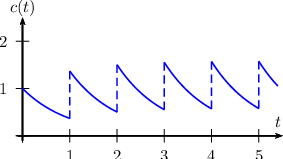
\includegraphics{figs/figura_dirac_12}\end{center}
 \caption{\label{concentracao}}
 \end{figure}
 O salto em cada descontinuidade é exatamente $c_0$, pois os limites laterais são
 \begin{eqnarray*}
 \lim_{t\to nT^-}c(t)&=&\lim_{t\to nT^-}\left(c_0e^{-\frac{t}{\tau}}\left(1+e^{\frac{T}{\tau}}+e^{\frac{2T}{\tau}}+\cdots+ e^{\frac{(n-1)T}{\tau}}\right)\right)\\
 &=&\left(c_0e^{-\frac{nT}{\tau}}\left(1+e^{\frac{T}{\tau}}+e^{\frac{2T}{\tau}}+\cdots+ e^{\frac{(n-1)T}{\tau}}\right)\right)\\
&=&\left(c_0\left(e^{-\frac{nT}{\tau}}+e^{-\frac{(n-1)T}{\tau}}+e^{-\frac{(n-2)T}{\tau}}+\cdots+ e^{-\frac{T}{\tau}}\right)\right)\\
\end{eqnarray*}
e
\begin{eqnarray*}
\lim_{t\to nT^+}c(t)&=&\lim_{t\to nT^+}\left(c_0e^{-\frac{t}{\tau}}\left(1+e^{\frac{T}{\tau}}+e^{\frac{2T}{\tau}}+\cdots+ e^{\frac{(n-1)T}{\tau}}+ e^{\frac{nT}{\tau}}\right)\right)\\
&=&\left(c_0e^{-\frac{nT}{\tau}}\left(1+e^{\frac{T}{\tau}}+e^{\frac{2T}{\tau}}+\cdots+ e^{\frac{(n-1)T}{\tau}}+ e^{\frac{nT}{\tau}}\right)\right)\\
&=&\left(c_0\left(e^{-\frac{nT}{\tau}}+e^{-\frac{(n-1)T}{\tau}}+e^{-\frac{(n-2)T}{\tau}}+\cdots+ e^{-\frac{T}{\tau}}+1\right)\right),\\
\end{eqnarray*}
 que possuem diferença igual a $c_0$. 
 Observe que quando calculamos o limite $\displaystyle \lim_{t\to 0^+}c(t)$ obtemos $c(0^+)=c_0$, valor diferente da condição inicial dada, que é $c(0)=0$. Apesar de parecer estranho, não está errado. Tudo é consequência da presença do Dirac em $t=0$, que produz uma discontinuidade na origem. Este assunto será discutido na seção \ref{problemas_na_origem}.
% % 
% % 
% % 
 \section{Problemas na origem}\label{problemas_na_origem}
 Para entender melhor esse fenômeno, vamos considerar um problema um pouco mais simples, dado pelo seguinte problema de valor inicial:
\begin{equation*}
\left\{
\begin{array}{rcl}
y'(t)+y(t)&=&\delta(t)\\
y(0)&=&0
\end{array}
\right.
\end{equation*}
Tomando a Transformada de Laplace, temos:
\begin{equation*}
sY(s)-y(0)+Y(s)=1
\end{equation*}
ou seja, $Y(s)=\frac{1}{s+1}$, o que implica
\begin{equation}y(t)=e^{-t}.\end{equation}
Observamos que $y(0)=1\neq 0$, ou seja, a condição inicial não é satisfeita.
Para entendermos o que está acontecendo, devemos lembrar que a Transformada de Laplace só produz a solução para $t>0$ e interpretar $y(t)$ como
\begin{equation}y(t)=u(t)e^{-t}.\end{equation}
Desta forma $y(0)$ simplesmente não está definido. De fato, para compreender esse comportamento, vamos definir um problema auxiliar colocando no lugar da função delta de Dirac uma função pulso:
\begin{equation*}
\left\{
\begin{array}{rcl}
y'(t)+y(t)&=&\frac{u(t)-u(t-\varepsilon)}{\varepsilon}\\
y(0)&=&0
\end{array}
\right.
\end{equation*}
onde $\varepsilon$ é uma constante positiva pequena. Sabemos que o termo \begin{equation}\frac{u(t)-u(t-\varepsilon)}{\varepsilon}\end{equation} converge para $\delta(t)$ quando $\varepsilon \to 0+$. Aplicando a Transformada de Laplace e resolvendo para $Y(s)$, temos:
\begin{equation}Y(s)=\frac{1}{s(s+1)}\frac{1-e^{-\varepsilon s}}{\varepsilon}=\left(\frac{1}{s}-\frac{1}{s+1}\right)\frac{1-e^{-\varepsilon s}}{\varepsilon},\end{equation}
ou seja,
\begin{equation}y(t)=\frac{1-e^{-t}}{\varepsilon}u(t)-u(t-\varepsilon)\frac{1-e^{-(t-\varepsilon)}}{\varepsilon}.\end{equation}
Esta solução pode ser escrita como uma função contínua:
\begin{equation}y(t)=\left\{\begin{array}{ll}
0,&t\leq 0,\\~\\
\frac{1-e^{-t}}{\varepsilon},&0<t\leq \varepsilon,\\~\\
\frac{e^{\varepsilon}-1}{\varepsilon}~\!
e^{-t},&t\geq \varepsilon.
\end{array}
\right.\end{equation}
Para $\varepsilon>0$ pequeno podemos usar a seguinte aproximação:
\begin{equation}e^t=1+t+\frac{t^2}{2}+\frac{t^3}{3!}+\ldots \approx 1+t\end{equation}
Assim, temos:
\begin{equation}y(t)\approx\left\{\begin{array}{ll}
0,&t\leq 0,\\~\\
\frac{t}{\varepsilon},&0<t\leq \varepsilon,\\~\\
e^{-t},&t\geq \varepsilon.
\end{array}
\right.\end{equation}
Ou seja, existe uma pequena região de transição entre $0$ e $\varepsilon$ onde a solução $y(t)$ sobe rapidamente. O gráfico apresentado na figura \ref{concentracao_2} mostra o comportamento de $y(t)$ para $\varepsilon=0.2$, $\varepsilon=0.1$ e $\varepsilon=0.05$ em azul, vermelho e verde, respectivamente, assim como a solução limite $e^{-t}u(t)$ em preto.
\begin{figure}[!ht]
\begin{center}

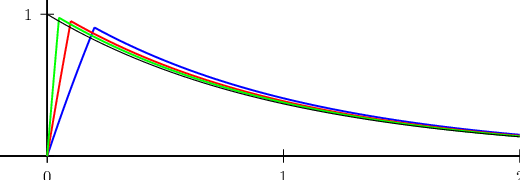
\includegraphics{figs/figura_dirac_13} \end{center}
\caption{\label{concentracao_2}}
 \end{figure}
 

 \chapter{2 de outubro}
 
 
\section{Propriedade da convolução}
Dada duas funções contínuas por partes em $[0,\infty]$, a convolução  de $f$ e $g$ denotada por $f*g$ é definida pela integral
\begin{equation}{\label{def_conv}}
 (f*g)(t)=\int_0^t f(\tau)g(t-\tau)d\tau.
\end{equation}

{\label{ex_conv_1}}Dadas $f(t)=e^t$ e $g(t)=\cos(t)$, vamos calcular $f*g$:
\begin{eqnarray*}
 (f*g)(t)&=&\int_0^t e^{\tau} \cos(t-\tau)d\tau\\
 &=&\left. \frac{1}{2}e^\tau\left(\cos(t-\tau)-\sin(t-\tau)  \right)\right|_0^t\\
 &=& \frac{1}{2}\left(e^t-\cos(t)+\sin(t)  \right).
\end{eqnarray*}
onde usamos que $\int  e^{\tau} \cos(t-\tau)d\tau=\frac{1}{2}e^\tau \left(\cos(t-\tau)-\sin(t-\tau)  \right)$+ constante.


{\label{prop_conv}}(Propriedade da convolução) Se $F(s)=\mathcal{L}\{f(t)\}$ e $G(s)=\mathcal{L}\{g(t)\}$, então
\begin{equation}{\label{eq_prop_conv}}
 \mathcal{L}\{(f*g)(t)\}=F(s)G(s).
\end{equation}
ou
\begin{equation}{\label{eq_inv_prop_conv}}
 \mathcal{L}^{-1}\{F(s)G(s)\}=(f*g)(t).
\end{equation}


 
Dem:
Partimos da definição das transformadas:
\begin{equation}
F(s)=\mathcal{L}\{f(t) \}=\int_0^\infty f(t)e^{-st}dt
\end{equation}
e
\begin{equation}
G(s)=\mathcal{L}\{g(\tau) \}=\int_0^\infty g(\tau)e^{-s\tau}d\tau.
\end{equation}
Logo,
\begin{eqnarray*}
 F(s)G(s)&=&\int_0^\infty f(t)e^{-st}dt\int_0^\infty g(\tau)e^{-s\tau}d\tau\\
&=&\int_0^\infty f(t) \int_0^\infty g(\tau)e^{-s(t+\tau)} d\tau dt\\
\end{eqnarray*}
Mantemos $t$ fixo e fazemos a mudança de variável $v=t+\tau$ para obter:
\begin{eqnarray*}
 F(s)G(s)=\int_0^\infty f(t) \int_t^\infty g(v-t)e^{-sv}dv dt\\
\end{eqnarray*}
Agora, vamos mudar a ordem de integração na região que é a metade inferior do primeiro quadrante: em vez de variar $v$ em $[t,\infty]$ depois $t$ em $[0,\infty]$, primeiro vamos variar $t$ em $[0,v]$, depois $v$ em $[0,\infty]$, ou seja,
\begin{eqnarray*}
 F(s)G(s)&=&\int_0^\infty  \int_0^v f(t) g(v-t)e^{-sv} dt dv\\
 &=&\int_0^\infty \left( \int_0^v f(t) g(v-t)dt\right)e^{-sv}  dv\\
 &=&\int_0^\infty (f*g)e^{-sv}  dv\\
   &=&\mathcal{L}\{f*g\}
\end{eqnarray*}


{\bf Exemplo} Vamos calcular a transformada inversa de $\frac{s}{(s-1)(s^2+1)}$. Primeiro observamos que a expressão pode ser escrita como um produto de duas funções tabelas:
\begin{equation}
\frac{s}{(s-1)(s^2+1)}=\frac{1}{s-1}\frac{s}{s^2+1},
\end{equation}
 onde $\mathcal{L}^{-1}\left\{\frac{1}{s-1}\right\}=e^t$ e $\mathcal{L}^{-1}\left\{\frac{s}{s^2+1}\right\}=\cos(t)$. Usando a propriedade \ref{prop_conv} da convolução, temos
 \begin{equation}
 \mathcal{L}^{-1}\left\{\frac{1}{s-1}\frac{s}{s^2+1}\right\}=\int_0^t e^\tau \cos(t-\tau)d\tau.
 \end{equation}
 A convolução acima foi calculada no exemplo \ref{ex_conv_1}, logo
\begin{equation}
 \mathcal{L}^{-1}\left\{\frac{1}{s-1}\frac{s}{s^2+1}\right\}= \frac{1}{2}\left(e^t-\cos(t)+\sin(t)  \right).
 \end{equation}
 
 
 
 A propriedade  da convolução pode ser útil para resolver equações integrais, como veremos no próximo exemplo.

 {\bf Exemplo:} Vamos resolver a seguinte equação integral:
 \begin{equation}
 y(t)=4+9\int_0^t y(\tau)(t-\tau)d\tau.
 \end{equation}
 Aplicamos a transformada de Laplace e usamos a propriedade \ref{prop_conv} da convolução com $f(t)=y(t)$ e $g(t)=t$ para obter:
 \begin{equation}
 \mathcal{L}\{y(t)\}=\frac{4}{s}+9\mathcal{L}\{y(t)\}\mathcal{L}\{t\}
 \end{equation}
 ou seja,
 \begin{equation}
 Y(s)=\frac{4}{s}+9Y(s)\frac{1}{s^2}.
 \end{equation}
 Logo,
 \begin{equation}
 Y(s)=\frac{s^2}{s^2-9}\frac{4}{s}=\frac{4s}{s^2-9}.
 \end{equation}
 Portanto,
 \begin{equation}
 y(t)=4\cosh(3t)
 \end{equation}


 \section{}
 
Nesse capítulo discutiremos a transformada de Laplace envolvendo funções especiais, tais como função de Bessel, função Gama e funções Seno Integrado. Também, desenvolveremos ferramentas capaz de resolver alguns problemas de valor iniciais com coeficientes não constantes.
Para iniciar as discussões vamos demonstrar o item 6 da tabela  no próximo exemplo.


{\bf Exemplo: }Vamos calcular a transformada de Laplace da funçao $t^{k-1}$, dada por:
\begin{equation}
\mathcal{L}\{t^{k-1} \}=\int_0^\infty t^{k-1} e^{-st}dt.
\end{equation}
Fazemos a mudança de variável $x=st$ para obter:
\begin{eqnarray*}
 \mathcal{L}\{t^{k-1} \}&=&\int_0^\infty \frac{x^{k-1}}{s^{k-1}}e^{-x}\frac{dx}{s}\\
 &=&\frac{1}{s^k}\int_0^\infty x^{k-1}e^{-x} dx.
 \end{eqnarray*}
A função que aparece acima é a multiplicação de $\frac{1}{s^k}$ por uma que não depende de $s$, chamada de função Gama e denotada por $\Gamma(k)$. Portanto, demonstramos o item 6 da tabela:
\begin{equation}
\mathcal{L}\{t^{k-1} \}=\frac{\Gamma(k)}{s^k},\qquad k>0,
\end{equation}
onde
\begin{equation}
\Gamma(k)=\int_0^\infty e^{-x}x^{k-1}dx.
\end{equation}


Observe que o item 3 da tabela é
\begin{equation}
\mathcal{L}\{t^{n-1}\}=\frac{(n-1)!}{s^n}, ~~  n\in \mathbb{N}.
\end{equation}
Isso nos indica que, para que os itens 3 e 6 sejam consistentes, $\Gamma(n+1)=n!$ se $n\in\mathbb{N}$. De fato, primeiro observe que, se $k=(n+1)\in\mathbb{N}$, temos:
\begin{equation}
\Gamma(n+1)=\int_0^\infty e^{-x}x^{n}dx=\left[-e^{-x}x^{n}\right]_0^\infty-\int_0^\infty (-e^{-x})nx^{n-1}dx=n\int_0^\infty e^{-x}x^{n-1}dx=n\Gamma(n).
\end{equation}
Como 
\begin{equation}
\Gamma(1)=\int_0^\infty e^{-x}dx=\left[-e^{-x}\right]_0^\infty=1,
\end{equation}
temos
\begin{equation}
\Gamma(2)=1,\qquad \Gamma(3)=2\cdot 1=2!,\qquad \Gamma(4)=3\Gamma(3)=3\cdot 2!=3!,\cdots
\end{equation}
Logo, $\Gamma(n+1)=n!$ se $n\in\mathbb{N}$.

{\bf Exemplo: } Os itens 4 e 5 da tabela são casos particulares do item 6:
 \begin{equation}
 \mathcal{L}\{t^{-\frac{1}{2}}\}=\frac{\Gamma\left(\frac{1}{2}\right)}{s^{\frac{1}{2}}}
 \end{equation}
e
 \begin{equation}
 \mathcal{L}\{t^{\frac{1}{2}}\}=\frac{\Gamma\left(\frac{3}{2}\right)}{s^{\frac{3}{2}}}.
 \end{equation}
 Basta calcular os valores de $\Gamma\left(\frac{1}{2}\right)$ e $\Gamma\left(\frac{3}{2}\right)$ para completar a demonstração. Começamos com $\Gamma\left(\frac{1}{2}\right)$:
 \begin{equation}
 \Gamma\left(\frac{1}{2}\right)=\int_0^\infty e^{-x}x^{-\frac{1}{2}}dx=\int_0^\infty \frac{e^{-x}}{\sqrt{x}}dx.
 \end{equation}
 Fazendo a mudança de variáveis $x=t^{2}$, obtemos $dx=2tdt$ e
\begin{equation}\Gamma\left(\frac{1}{2}\right)=2\int_{0}^{\infty}e^{-t^2}dt
\end{equation}
Utilizando a técnica de Liouville, definimos:
\begin{equation}
I=\int_{0}^{\infty}e^{-t^2}dt
\end{equation}
Logo
\begin{equation}
I^2=\int_{0}^{\infty}e^{-x^2}dx\int_{0}^{\infty}e^{-y^2}dy=\int_{0}^{\infty}\int_{0}^{\infty}e^{-(x^2+y^2)}dx dy
\end{equation}
A última integral é uma integral dupla que pode ser calculada em coordenadas polares fazendo $r^2=x^2+y^2$ e $dxdy=rdrd\theta$:
\begin{equation}
I^2=\int_{0}^{\frac{\pi}{2}}\int_{0}^{\infty}e^{-r^2}rdr d{\theta}=\frac{\pi}{2}\left[-\frac{e^{-r^2}}{2}\right]_0^\infty=\frac{\pi}{4}
\end{equation}
Assim,
\begin{equation}
I^2=\frac{\pi}{4}\Rightarrow I=\frac{\sqrt{\pi}}{2}
\end{equation}
e
\begin{equation}
\Gamma\left(\frac{1}{2}\right)=2\int_{0}^{\infty}e^{-t^2}dt=2I=\sqrt{\pi}.
\end{equation}
Agora, usando a propriedade da função Gama que $\Gamma(k+1)=k\Gamma(k)$, temos:
\begin{equation}
\Gamma\left(\frac{3}{2}\right)=\frac{1}{2}\Gamma\left(\frac{1}{2}\right)=\frac{\sqrt{\pi}}{2}.
\end{equation}
Portanto, os itens 4 e 5 da tabela são válidos:
\begin{equation}
 \mathcal{L}\{t^{-\frac{1}{2}}\}=\frac{\sqrt{\pi}}{\sqrt{s}}
\end{equation}
e
\begin{equation}
 \mathcal{L}\{t^{\frac{1}{2}}\}=\frac{\sqrt{\pi}}{2s^{\frac{3}{2}}}.
\end{equation}
 
 {\bf Exemplo: }Vamos calcular a transformada de Laplace da função $\ln(t)$ (item 38 da tabela). Com esse objetivo, usamos a transformada de Laplace de $t^k$ dada no item 6 da tabela:
\begin{equation}
\int_0^\infty t^ke^{-st}dt=\frac{\Gamma(k+1)}{s^{k+1}}.
\end{equation}
Agora, como o integrando do lado esquerdo é uma função contínua e tem derivada parcial com respeito a $k$ contínua podemos diferenciar ambos os lados com respeito ao parâmetro $k$ usando a regra de Leibniz
\begin{eqnarray*}
\frac{d}{dk}\left(\int_0^\infty t^ke^{-st}dt\right)&=&\frac{d}{dk}\left(\frac{\Gamma(k+1)}{s^{k+1}}\right)\\
&\Downarrow&\\
\int_0^\infty t^k \ln(t) e^{-st}dt&=&\frac{s^{k+1}\Gamma'(k+1)-\Gamma(k+1)s^{k+1}\ln(s)}{s^{2(k+1)}}
\end{eqnarray*}
Agora, fazemos $k\to 0$ para obter
\begin{equation}
\int_0^\infty \ln(t) e^{-st}dt=\frac{s^{1}\Gamma'(1)-\Gamma(1)s^{1}\ln(s)}{s^{2}},
\end{equation}
ou seja,
\begin{equation}
\int_0^\infty \ln(t) e^{-st}dt=\frac{\Gamma'(1)-\ln(s)}{s},
\end{equation}
já que $\Gamma(1)=1$. Do lado esquerdo aparece a transformada da função $\ln(t)$ e do lado direito $\Gamma'(1)$. Então calculamos
\begin{equation}
\Gamma'(k)=\int_0^\infty x^{k-1}\ln(x) e^{-x}dx
\end{equation}
e
\begin{equation}
\Gamma'(1)=\int_0^\infty \ln(x) e^{-x} dx=-\gamma
\end{equation}
where $\gamma$ é a constante de Euler - Mascheroni,
\begin{equation}
\gamma=0.57721566490153286060651209008240243104215933593992\cdots.
\end{equation}
Finalmente, concluímos
\begin{equation}
\mathcal{L}\{\ln(t)\}=\frac{-\gamma-\ln(s)}{s}
\end{equation}

%%%%%%%%%%%%%%%%%%%%%%%%%%%%%%%%%%%%%%%%%%%%%%%%%%%%%%


\section{Transformada de Laplace de funções periódicas}
Nesta seção apresentaremos uma propriedade da transformada de Laplace de funções periódicas e calcularemos algumas delas.

 Seja $f(t)$ uma função contínua por partes e periódica de período $T$. Então sua transformada de Laplace é da forma
\begin{equation}
\mathcal{L}\{f(t)\}=\frac{1}{1-e^{-sT}}\int_0^Tf(t)e^{-st}dt.
\end{equation}


Dem: Aplicamos a definição e separamos a integral nos períodos da função $f(t)$ para obter:
\begin{eqnarray*}
 \mathcal{L}\{f(t)\}&=&\int_0^\infty f(t)e^{-st}dt \\
 &=&\int_0^T f(t)e^{-st}dt+\int_T^{2T} f(t)e^{-st}dt+\int_{3T}^{4T} f(t)e^{-st}dt+\cdots\\
 &=&\sum_{n=0}^\infty \int_{nT}^{(n+1)T} f(t)e^{-st}dt.
\end{eqnarray*}
Fazemos a mudança de variável $\tau=t-nT$ e obtemos
 \begin{eqnarray*}
 \mathcal{L}\{f(t)\}&=&\sum_{n=0}^\infty \int_{0}^{T} f(\tau+nT)e^{-s(\tau+nT)}d\tau\\
 &=&\sum_{n=0}^\infty e^{-snT} \int_{0}^{T} f(\tau+nT)e^{-s\tau}d\tau.
 \end{eqnarray*}
 Usando o fato que a função é periódica, ou seja, $f(\tau)=f(\tau+nT)$, temos:
 \begin{eqnarray*}
  \mathcal{L}\{f(t)\}&=&\sum_{n=0}^\infty e^{-snT} \int_{0}^{T} f(\tau)e^{-s\tau}d\tau\\
 &=&\int_{0}^{T} f(\tau)e^{-s\tau}d\tau\left[\sum_{n=0}^\infty \left(e^{-sT}\right)^n \right]\\
 &=&\int_{0}^{T} f(\tau)e^{-s\tau}d\tau\left[\frac{1}{1-e^{-sT}} \right]\\
 &=&\frac{1}{1-e^{-sT}}\int_{0}^{T} f(\tau)e^{-s\tau}d\tau,
\end{eqnarray*}
onde usamos a soma de uma série geométrica de razão $e^{-sT}$.
 
 
{\bf Exemplo} Observe o cálculo da transformada da função $f(t)=\cos(wt)$ sabendo que
\begin{equation}
\int \cos(wt)e^{-st}dt=\frac{e^{-st}\left(w\sin(wt)-s\cos(wt)\right)}{s^2+w^2}+\ \!\hbox{Constante}
\end{equation}
e usando a propriedade \ref{prop_fun_per}:
\begin{eqnarray*} 
\mathcal{L}\{\cos(wt)\}&=&\frac{1}{1-e^{-s\frac{2\pi }{w}}}\int_0^{\frac{2\pi }{w}}\cos(wt)e^{-st}dt\\
&=&\frac{1}{1-e^{-s\frac{2\pi }{w}}}\left[\frac{e^{-st}\left(w\sin(wt)-s\cos(wt)\right)}{s^2+w^2}\right]_0^{\frac{2\pi }{w}}\\
&=&\frac{1}{1-e^{-s\frac{2\pi }{w}}}\frac{s-se^{-s\frac{2\pi }{w}}}{s^2+w^2}\\
&=&\frac{s}{s^2+w^2}.
\end{eqnarray*}


{\bf Exemplo} A função $f(t)$ apresentada no gráfico da figura \ref{fig_onda_quadrada} é chamada de {\bf onda quadrada} de período $2a$.
 \begin{figure}[!ht]
\begin{center}

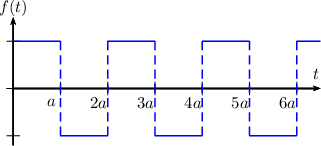
\includegraphics{figs/especiais_figura_1}\end{center}
\caption{\label{fig_onda_quadrada}}
\end{figure}
Calculamos a transformada de Laplace usando a propriedade \ref{prop_fun_per} colocando $T=2a$
\begin{eqnarray*}
\mathcal{L}\{f(t)\}&=& \frac{1}{1-e^{-2sa}}\int_0^{2a}f(t)e^{-st}dt\\
&=& \frac{1}{1-e^{-2sa}}\left(\int_0^{a}e^{-st}dt-\int_a^{2a}e^{-st}dt\right)\\
&=& \frac{1}{1-e^{-2sa}}\left(\frac{1-2e^{-as}+e^{-2as}}{s}\right)\\
&=& \frac{1}{(1-e^{-sa})(1+e^{-sa})}\left(\frac{(1-e^{-as})^2}{s}\right)\\
&=&\frac{1}{s} \frac{1-e^{-as}}{1+e^{-sa}}.\\
\end{eqnarray*}
Multiplicando por $e^{\frac{as}{2}}$, podemos escrever a expressão em termos de funções hiperbólicas:
\begin{eqnarray*}
\mathcal{L}\{f(t)\}&=&\frac{1}{s} \frac{e^{\frac{as}{2}}-e^{-\frac{as}{2}}}{e^{\frac{as}{2}}+e^{-\frac{as}{2}})}\\
&=&\frac{1}{s} \frac{\sinh\left(\frac{as}{2}\right)}{\cosh\left(\frac{as}{2}\right)}\\
&=&\frac{1}{s} \tanh\left(\frac{as}{2}\right).
\end{eqnarray*}

 
A função $g(t)$ apresentada no gráfico da figura  é chamada de {\bf onda triangular} de perído $2a$.
\begin{figure}[!ht]
 \begin{center}
 
 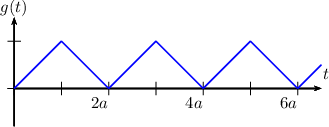
\includegraphics{figs/especiais_figura_2}\end{center}
 \caption{\label{fig_onda_triangular}}
 \end{figure}
 Para calcular a transformada de Laplace, observe que:
 \begin{itemize}
  \item[a)] A função $g(t)$ representada na figura  tem como derivada uma onda quadrada. De fato, no intervalo $[0,a]$, a derivada é $\frac{1}{a}$ e no intervalo $[a,2a]$ a derivada é $-\frac{1}{a}$. Esse padrão se repete periodicamente. Logo, a derivada da onda triangular é a onda quadrada multiplicada por $\frac{1}{a}$.
  \item[b)] Temos:
  \begin{equation}
  \mathcal{L}\{g(t)\}=\frac{1}{s}\mathcal{L}\{g'(t)\}+\frac{1}{s}g(0).
  \end{equation}
 \end{itemize}
 Logo,
 \begin{eqnarray*}
 \mathcal{L}\{\hbox{onda triangular}\}&=&\frac{1}{as}\mathcal{L}\{\hbox{onda quadrada}\}+\frac{1}{s}\hbox{(onda triangular na origem)},
 \end{eqnarray*}
 e, portanto, usando o fato que a onda triangular vale zero na origem e o resultado do exemplo, temos
 \begin{eqnarray*}
 \mathcal{L}\{g(t)\}&=&\frac{1}{as}\frac{1}{s} \tanh\left(\frac{as}{2}\right)\\
 &=&\frac{1}{as^2} \tanh\left(\frac{as}{2}\right).
 \end{eqnarray*}

{\bf Exemplo} A função $h(t)$ dada por
\begin{equation}
h(t)=\left\{\begin{array}{ll}\sin(wt),&0<t<\frac{\pi}{w}\\0,& \frac{\pi}{w}<t<\frac{2\pi}{w}, \end{array}\right.,
\end{equation}
$h\left(t+\frac{2\pi}{w}\right)=h(t)$, é chamada de {\bf retificador de meia onda} de período $\frac{2\pi}{w}$. A figura \ref{fig_ret_meia_onda} apresenta o gráfico da função $h(t)$.
  \begin{figure}[!ht]
 \begin{center}
  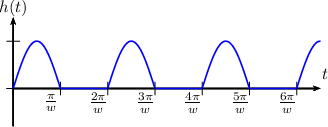
\includegraphics{figs/especiais_figura_3}
  \end{center}
  \caption{\label{fig_ret_meia_onda}}
 \end{figure}

Calculamos a transformada de Laplace usando a propriedade \ref{prop_fun_per} com $T=\frac{2\pi}{w}$
\begin{eqnarray*}
\mathcal{L}\{f(t)\}&=& \frac{1}{1-e^{-s\frac{2\pi}{w}}}\int_0^{\frac{2\pi}{w}}f(t)e^{-st}dt\\
&=& \frac{1}{1-e^{-s\frac{2\pi}{w}}} \int_0^{\frac{\pi}{w}}\sin(wt)e^{-st}dt\\
&=& \frac{1}{1-e^{-s\frac{2\pi}{w}}} \left[-\frac{e^{-st}\left(s\sin(wt)+w\cos(wt)\right)}{s^2+w^2}\right]_0^{\frac{\pi}{w}}\\
&=& \frac{1}{(1-e^{-\frac{s\pi}{w}})(1+e^{-\frac{s\pi}{w}})} \frac{w(1+e^{-\frac{s\pi}{w}})}{s^2+w^2}\\
&=& \frac{1}{1-e^{-\frac{s\pi}{w}}} \frac{w}{s^2+w^2}
\end{eqnarray*}

{\bf Exemplo:} A função $p(t)$ dada por
\begin{equation}
p(t)=|\sin(wt)|
\end{equation}
 é chamada de {\bf retificador de onda completa} de período $\frac{\pi}{w}$. A figura \ref{fig_ret_onda_completa} apresenta o gráfico da função $p(t)$.
  \begin{figure}[!ht]
 \begin{center}
% 
 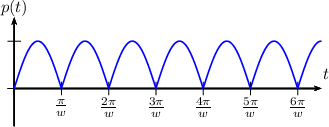
\includegraphics{figs/especiais_figura_4}\end{center}
 \caption{\label{fig_ret_onda_completa}}
 \end{figure}
 Calculamos a transformada de Laplace usando a propriedade \ref{prop_fun_per} com $T=\frac{\pi}{w}$
 \begin{eqnarray*}
 \mathcal{L}\{p(t)\}&=& \frac{1}{1-e^{-s\frac{\pi}{w}}}\int_0^{\frac{\pi}{w}}\sin(wt)e^{-st}dt\\
 &=& \frac{1}{1-e^{-s\frac{\pi}{w}}} \left[-\frac{e^{-st}\left(\sin(wt)+w\cos(wt)\right)}{s^2+w^2}\right]_0^{\frac{\pi}{w}}\\
 &=& \frac{1}{1-e^{-\frac{s\pi}{w}}} \frac{w(1+e^{-\frac{s\pi}{w}})}{s^2+w^2}\\
 &=&  \frac{w}{s^2+w^2}\frac{e^{\frac{s\pi}{2w}}+e^{-\frac{s\pi}{2w}}}{e^{\frac{s\pi}{2w}}-e^{-\frac{s\pi}{2w}}}\\
 &=&  \frac{w}{s^2+w^2}\coth\left( \frac{\pi s}{2w}\right)
 \end{eqnarray*}

{\bf Exemplo:} A função $q(t)$ dada por
 \begin{equation}
 \left\{\begin{array}{ll}q(t)=\frac{t}{a},&0\leq t<a\\ q\left(t+a\right)=q(t), & \end{array}\right.
 \end{equation}
 é chamada de {\bf onda dente de serra} de período $T=a$. A figura \ref{fig_dente_de_serra} apresenta o gráfico da função $q(t)$.
  \begin{figure}[!ht]
 \begin{center}
 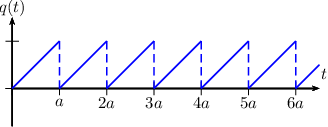
\includegraphics{figs/especiais_figura_5}
 \end{center}
 \caption{\label{fig_dente_de_serra}}
 \end{figure}
 Calculamos a transformada de Laplace usando a propriedade  com $T=a$:
 \begin{eqnarray*}
 \mathcal{L}\{q(t)\}&=& \frac{1}{1-e^{-sa}} \int_0^{a} \frac{t}{a} e^{-st}dt\\
 &=&\frac{1}{1-e^{-sa}}\frac{1}{a}\left[ -\frac{e^{-s t} (1+s t)}{s^2}\right]_0^a\\
 &=&\frac{1}{1-e^{-sa}}\frac{1-e^{-sa}(1+as)}{s^2a} \\
 &=&\frac{1}{1-e^{-sa}}\left(\frac{1-e^{-sa}-e^{-sa} as)}{s^2a} \right)\\
 &=&\frac{1}{as^2}-\frac{e^{-sa} }{s\left(1-e^{-sa}\right)}.
 \end{eqnarray*}


 \section{Propriedades do Valor Inicial e Final}
 Se $F(s)$ é a transformada de Laplace de $f(t)$ e 
\begin{equation}
\lim_{t\to\infty}f(t)=L,
\end{equation}
então
\begin{equation}
\lim_{s\to 0^+} sF(s)=L.
\end{equation}

Dem: Usamos a definição de transformada de Laplace para escrever
\begin{eqnarray*}
sF(s)&=&s\int_0^\infty f(t)e^{-st}dt\\
&=&s\int_0^a f(t)e^{-st}dt+s\int_a^\infty f(t)e^{-st}dt.\\
\end{eqnarray*}
Observe que a primeira parcela do lado direito tende a zero independentemente do valor de $a$. Porém, para $a$ suficientemente grande, $f(t)$ se aproxima de $L$, pois $\displaystyle \lim_{t\to\infty}f(t)=L$, ou seja,
\begin{eqnarray*}
s\int_a^\infty f(t)e^{-st}dt &\approx &s\int_a^\infty L e^{-st}dt.\\
&\approx &s\frac{L}{-s}\left[ e^{-st}\right]_a^\infty=Le^{-as}
\end{eqnarray*}
Como $e^{-as}\to 1$ quando $s\to 0$, então
\begin{equation}
\lim_{s\to 0^+} sF(s)=L.
\end{equation} 




Se $F(s)$ é a transformada de Laplace de uma função $f(t)$ de ordem exponencial $c$ e 
\begin{equation}
\lim_{t\to 0^+}f(t)=L,
\end{equation}
então
\begin{equation}
\lim_{s\to \infty} sF(s)=L.
\end{equation}

Dem: Usamos a definição de transformada de Laplace para escrever
\begin{eqnarray*}
sF(s)&=&s\int_0^\infty f(t)e^{-st}dt\\
&=&s\int_0^a f(t)e^{-st}dt+s\int_a^b f(t)e^{-st}dt+s\int_b^\infty f(t)e^{-st}dt.\\
\end{eqnarray*}
Observe que a segunda parcela do lado direito tende a zero quando $s\to \infty$ independentemente do valor de $a$ e $b$, pois o fato da função ser de ordem exponencial e contínua por partes implica em $f(t)$ limitada em $[a,b]$, ou seja, $|f(t)|<M$ e, portanto,
\begin{eqnarray*}
\left|s\int_a^b f(t)e^{-st}dt\right|&\leq & s\int_a^b |f(t)|e^{-st}dt\\
&\leq & Ms\int_a^b e^{-st}dt\\
&\leq & \left.Ms\frac{1}{-s} e^{-st}\right|_a^b=M(e^{-sa}-e^{-sb}).
\end{eqnarray*}
Também, a terceira parcela tende a zero se $b$ for suficientemente grande, pois existem $c$ e $M>0$ tal que $|f(t)|<Me^{ct}$ para $t>b$ e, portanto,
\begin{eqnarray*}
\left|s\int_b^\infty f(t)e^{-st}dt\right|&\leq & s\int_b^\infty |f(t)|e^{-st}dt\\
&\leq & s\int_b^\infty Me^{-(s-c)t}dt\\
&\leq & \left.Ms\frac{1}{c-s} e^{-(s-c)t}\right|_b^\infty=\frac{Ms}{s-c}(e^{-(s-c)b}).
\end{eqnarray*}
Porém, para $a$ suficientemente pequeno, $f(t)$ se aproxima de $L$, pois $\displaystyle \lim_{t\to 0}f(t)=L$, ou seja,
\begin{eqnarray*}
s\int_0^a f(t)e^{-st}dt &\approx &s\int_0^a L e^{-st}dt.\\
&\approx &s\frac{L}{-s}\left[ e^{-st}\right]_0^a=L\left(1-e^{-as}\right)
\end{eqnarray*}
Como $e^{-as}\to 0$ quando $s\to \infty$, então
\begin{equation}
\lim_{s\to \infty} sF(s)=L.
\end{equation} 

\section{Sistemas}
%O problema do forno.
% 
% 
% % 
% % 
% % 
% %                             
% %                             
\end{document}
  
